\begin{frame}{Conversão de Sistema de Efeitos para Mônadas}
    \begin{itemize}
        \item A correspondência entre sistema de efeitos e mônadas foi observada por \citeonline{wadler2003marriage}.

        \item Seguindo essa abordagem, \citeonline{vazou2016monads} formalizam a tradução do sistema de efeitos de Koka para mônadas.

        \item[] 

        \item [] \begin{figure}
            \centering
            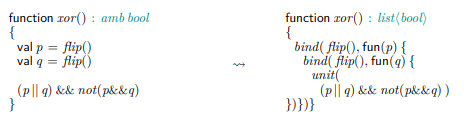
\includegraphics[width=.9\textwidth]{Figuras/conv.png}
            \caption{Exemplo de Tradução da Função \textit{xor} \cite{vazou2016monads}}
            \label{fig:conv1}
        \end{figure}
    \end{itemize}
\end{frame}

\begin{frame}{Conversão de Sistema de Efeitos para Mônadas}
    \begin{itemize}
        \item Para lidar com polimorfismo, cada função que utiliza efeitos polimórficos recebe um dicionário como argumento extra. O dicionário vai encontrar e retornar as funções de \textit{unit} e \textit{bind} correspondentes ao efeito gerado.

        \item Nos casos onde existe a necessidade de traduzir uma função com mais de um efeito (\textit{row-effects}), uma mônada é criada para representar a junção destes efeitos. Morfismos de \textit{lifting} de cada mônada de efeito para a mônada de junção também são criados.
    \end{itemize}
\end{frame}
    % easter egg = Brian
% \begin{frame}{Exemplo de Conversão de Row-Effect}
%     Digamos que existam dois efeitos \textit{IO} e \textit{amb} já definidos e uma função $f$ cujo efeito gerado é $\langle IO, amb \rangle$. Neste caso, uma mônada \textit{IOamb} e as funções \textit{IO2IOamb} e \textit{amb2IOamb} são criadas, de modo que \textit{IO2IOamb} recebe uma mônada \textit{IO} e retorna uma mônada \textit{IOamb} e \textit{amb2IOamb} recebe uma mônada \textit{amb} e retorna uma mônada \textit{IOamb}.
% \end{frame}